\documentclass[sigconf,authordraft]{acmart}

\usepackage{gensymb}
\usepackage[inline,shortlabels]{enumitem}
\usepackage{amsmath}
\usepackage{graphicx}

\AtBeginDocument{%
  \providecommand\BibTeX{{%
    \normalfont B\kern-0.5em{\scshape i\kern-0.25em b}\kern-0.8em\TeX}}}

\citestyle{acmauthoryear}

\begin{document}

\title{Application of Reinforcement Learning in NASA Swarmathon Competition}

\author{Rolando J. Nieves}
\email{rolando.j.nieves@knights.ucf.edu}
\authornotemark[1]
\affiliation{%
  \institution{University of Central Florida}
  \streetaddress{4000 Central Florida Blvd.}
  \city{Orlando}
  \state{Florida}
  \postcode{32816}
}

\renewcommand{\shortauthors}{Nieves}

\begin{abstract}
  The NASA Swarmathon competition domain provides an excellent proving ground
  for the implementation of multi-agent cooperative behavior using Reinforcement
  Learning (RL). This report documents the results of a study aimed at replacing
  the fixed, swarm-like logic offered as a baseline to competition entrants with
  a system that can be trained in a simulated environment prior to deployment
  onto an entrant's physical robots.
\end{abstract}

\begin{CCSXML}
  <ccs2012>
    <concept>
      <concept_id>10010147.10010178.10010219.10010220</concept_id>
      <concept_desc>Computing methodologies~Multi-agent systems</concept_desc>
      <concept_significance>500</concept_significance>
    </concept>
    <concept>
      <concept_id>10010147.10010257.10010258.10010261.10010275</concept_id>
      <concept_desc>
        Computing methodologies~Multi-agent reinforcement learning
      </concept_desc>
      <concept_significance>500</concept_significance>
    </concept>
  </ccs2012>
\end{CCSXML}

\ccsdesc[500]{Computing methodologies~Multi-agent systems}
\ccsdesc[500]{Computing methodologies~Multi-agent reinforcement learning}

\keywords{multi-agent systems,machine learning,reinforcement learning}

\begin{teaserfigure}
  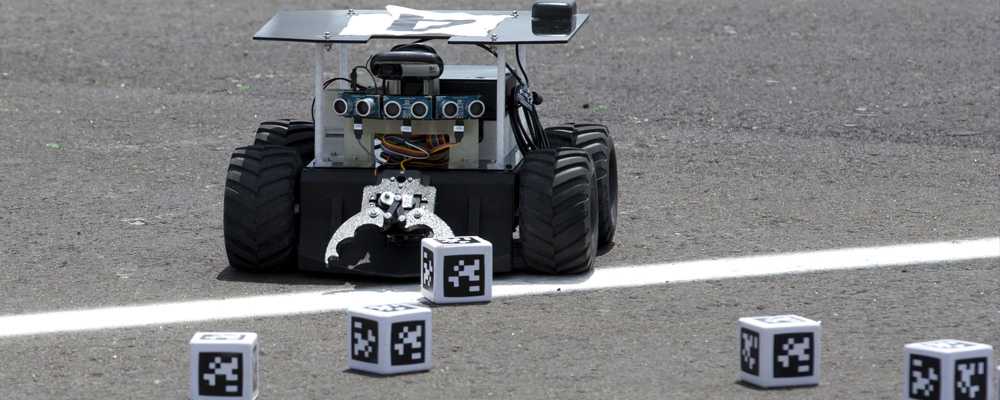
\includegraphics[width=\textwidth]{images/swarmathon-teaser.jpg}
  \caption{Montgomery College ``Swarmie'' in 2017 NASA Swarmathon}
  \Description{Image of a robotic member of the Montgomery College Swarmathon team entrant competing in NASA Swarmathon 2017}
  \label{fig:teaser}
\end{teaserfigure}

\maketitle

\section{Introduction}\label{sec:intro}
The study of applying Reinforcement Learning (RL) into cooperative multi-agent
systems remains a hot topic at the time of this writing. The topic's popularity
owes primarily to the fact that, unlike single agent RL, no single system
architecture has yet emerged as clearly superior among all available options.
Current architectural patterns such as Independent Learners (IL) and
Joint-Action Learners (JAL) exhibit traits that in some environments prove
quite beneficial. In other environments, however, these same traits represent
intolerable liabilities.

Thus, the search for a ``better mouse trap'' in the area of cooperating,
multi-agent RL has led to a proliferation of problem domains under which
methodology performance can be tested and quantified. From grid-world like
synthetic predator-prey scenarios, to more flexible environments like RoboCup
2D Simulated Soccer, these domains offer efficient ways to test theories. One
shortcoming of these problem domains, however, is the difficulty of implementing
any realized achievements into a physical domain.

The NASA Swarmathon problem domain offers an exciting opportunity for research
in this field. This is so because, combined with a robust simulation environment
based around the Robot Operating System (ROS) software suite, the domain offers
a clear path to implementation into physical robots participating in live
competition.

\section{Problem Domain}\label{sec:prob_domain}
In a generic sense, NASA Swarmathon is a resource gathering exercise using a
swarm of autonomous robots. The robotic swarm is expected to gather a set of
resources from their surrounding environment onto a collection area without
relying on any human supervision. NASA's intent with the competition is the
development of technologies that could one day be used to deploy ``advance
missions'' that perform as much preparation as possible at a planetary body site ahead of the arrival by human explorers.

NASA defines the Swarmathon competition environment using the following
elements:

\begin{itemize}
  \item A $16 \times 16$ or $32 \times 32$ meter square field where the
  competition takes place. The field size varies based on the round the
  competition is at.
  \item A swarm of three or six robots, with each robot labeled as a
  ``swarmie.''
  \item Up to 256, $2 \times 2 \times 2$ inch cubes bearing ``April Tag''
  markers on all six faces, known as April Cubes.
  \item A $1 \times 1$ meter square collection area within the competition
  field, known as a ``nest.''
\end{itemize}

During a competition round, a set of April Cubes are randomly strewn across
open areas of the competition field (i.e., no cubes initially start at
the ``nest''). The robotic swarm is then tasked with collecting the cubes onto
the ``nest.'' The periphery of the nest is labeled using another set of ``April
Tags,'' serving as a visual indicator for the robots. Collected cubes must be
in contact with the ``nest'' in order for them to count towards the team's
overall score.

Team members are not allowed contact or communication with the robots
(``swarmies'') during a round, leaving the robots to complete the task
leveraging their built-in sensor package and logic deployed to them prior to the
round. Individual robots are, however, allowed to communicate amongst
themselves. Although no restrictions on underlying physical communication fabric
exists as of this writing, the selected physical fabric must be exposed to the
robots via the ROS Publish-Subscribe communication system. A popular choice among teams is the use of Wi-Fi networking to implement robot-to-robot communication. No restrictions regarding bandwidth or reliability is imposed on the teams as of this writing.

\subsection{Sensor Package}\label{subsec:sensors}
The elements that comprise the ``swarmie'' sensor package include the
following:

\begin{itemize}
  \item Three ultrasonic range finders able to detect obstacles up to 3 meters
  away. The sensors are located in front of the robot, and evenly distributed
  across a $60^{\circ}$ arc.
  \item One Inertial Measurement Unit (IMU) used to estimate robot orientation
  and, in combination with other sensors, robot pose in the fixed competition
  area.
  \item One camera emitting color $320 \times 240$ resolution images at about
  six frames per second (FPS).
  \item One Global Positioning Satellite (GPS) receiver emitting latitude and
  longitude readings that, in combination with other sensors, help establish the
  robot's pose in the competition area.
  \item One odometer emitting wheel movement that, in combination with other
  sensors, help establish the robot's pose in the competition area.
\end{itemize}

In order to combine, or ``fuse,'' several of the sensor readings into a complete
robot pose, the baseline software provided by NASA includes an Extended Kalman
Filter (EKF) pipeline that eventually produces the following pose information:

\begin{itemize}
  \item Cartesian $(x,y,z)$ position with (albeit mostly static) altitude.
  \item Yaw with respect to a fixed reference frame.
  \item Linear $(x,y)$ velocity.
  \item Angular velocity about the Yaw axis
  \item Linear $(x,y)$ acceleration. 
\end{itemize}

Given that the robots are four-wheeled traversing a flat area, linear velocity
and acceleration in the altitude $z$ axis, as well as angular position and
velocity about the Roll and Pitch axes is not calculated.

The NASA baseline software also includes computer vision (CV) facilities that, when
combined with the camera and robot pose calculations, are able to provide
information about any ``April Tags'' visible within the robot's field of view.
As stated previously, the April Cubes that the robots must gather are
labeled on all six faces with the aforementioned tags, as is the ``nest''
periphery where the robots must deposit the cubes.

The NASA baseline software is written in terms of the facilities and services
provided by ROS, particularly when it comes to communication. Software provided
by teams must run within ROS and, again, may only utilize the Publish-Subscribe
system provided with ROS for their communication needs. In addition, the NASA
baseline software provides a simulation environment that combines ROS Gazebo
with 3D models of the robots and sensor emulation. During a simulation session,
the communication traffic fed as input to the software components that combine
to implement a robot's logic is practically indistinguishable from traffic that
would be produced by the sensor package of a physical robot.

\section{Related Works}\label{sec:related_works}
Reinforcement Learning (RL) is the approach that facilitates the creation of an action selection policy that is refined via direct interactions with the host environment. Combining pertinent information from the environment, along with a set of rewards or penalties gained performing different actions, the approach aims to yield an ever improving policy. The improvement of this policy is directly measured by the rewards gained during interactions with the environment. Expressed mathematically, given a set of pertinent environment traits combined into a state specification $s \in S$, with a set of state-dependent actions $a \in A(s)$, RL aims to maximize the state value function $v(s)$, as seen in Equation \ref{eq:state_value}.

\begin{equation}
  \label{eq:state_value}
  v_*(s) = \max_{a \in A(s)} q_{\pi *}(s, a)
\end{equation}

The state value function is dependent on the state-action function $q_\pi(s,a)$. Assuming a Markovian environment, the state-action function can be expressed in the form of a \textit{Bellman Optimality Equation} as shown in Equation \ref{eq:action_value_bellman}.

\begin{equation}
  \label{eq:action_value_bellman}
  q_{\pi *}(s, a) = \sum_{s', r} p(s', r | s, a) [r + \gamma \max_{a'}q_{\pi *}(s',a')]
\end{equation}

One of the algorithms used to implement RL that has yielded quite impressive results as of late is Deep Q-Networks (DQN) as originally outlined by \cite{mnih2015human}. The algorithm as designed by Mnih uses deep neural networks to produce action selection scores based solely on observed system state. The algorithm scales well from a low-dimensionality problem like the one explored in this study, to a far more complex problem such as the domain presented in the aforementioned work, where the algorithm learned to play Atari games by observing the screen output.

During training, the algorithm actually calls for the creation of two neural networks with identical architecture. One network (referred to here as the ``main'' network) is used to select an action based on the given system state. Another network (referred to here as the ``target'' network) is used to evaluate the selection made by the ``main'' network. The condition that Mnih was trying to mitigate with this approach is the use of a single network for both action selection and evaluation. Keeping the ``target'' network relatively intact during training, save for some periodic synchronizations, helps mitigate the over-estimation that had been observed with Q-Learning, which sometimes led to sub-optimal policies.

Another RL algorithm that would have been a good fit for this problem is the SARSA($\lambda$) algorithm as offered by \cite{sutton2018reinforcement}. SARSA($\lambda$) offered good policy learning performance in a computationally economical form. Application of the algorithm on multi-agent systems has seen wide success, such as that documented in \cite{keepaway-stone2006}. A challenge that remained with SARSA($\lambda$), however, is that prior to input the system state vector must be combined with an action vector in order to create what Sutton refers to a ``feature vector.'' Some texts, including Sutton's, provide examples with engineered state to feature vector conversions. Stone in his work avoided the use of engineered feature vectors by transforming the state vector using tile coding. The ease of use of DQN compared to SARSA($\lambda$) made it the better choice in the opinion of this author.

\section{Methodology}\label{sec:methodology}

\subsection{Challenges}\label{subsec:challenges}
There are many aspects of the NASA Swarmathon domain that pose a challenge against the implementation of a Reinforcement Learning (RL) based solution. Chief among these challenges are:

\begin{itemize}
  \item Although the number of April Cubes the Swarmies are tasked with foraging is fixed and known, their exact location in the arena is not.
  \item The Swarmies identify the location of April Cubes using two-dimensional cartesian coordinates $\textbf{L} \in \mathbb{R}^2$ based on the coordinate reference frame individually maintained by each Swarmie.
  \item The Swarmies navigate the competition area primarily using waypoints that are specified as two-dimensional cartesian coordinates $\textbf{W} \in \mathbb{R}^2$, again based on the individual reference frame maintained by each Swarmie.
  \item The Swarmies are not designed to properly map the competition area, thus they are required to continuously detect and properly react to the area's boundaries as well as the collection ``nest.''
\end{itemize}

Addressing each one of the aforementioned challenges is not impossible, but does impact the RL-based solution in ways that could introduce some margin of error and uncertainty.

\subsection{Shared Localization}\label{subsec:localization}
The lack of persistent mapping capability by the Swarmies poses a significant challenge, since actions within and around several very important landmarks (such as the collection zone or ``nest'') have material consequences towards the ultimate goal of the exercise. In addition, using a consistent reference frame for communicating location information amongst the swarm (be it latest robot position or April Cube sightings) is paramount. Section \ref{subsec:localization} details the methodology implemented to address this challenge.

Considered in isolation, the requirement that the robotic swarm find the location of all the April Cubes with very little prior knowledge is not a very difficult problem. Indeed, such a problem closely resembles a run-of-the-mill mapping exercise. The complications begin to arise once the following facts are taken into consideration:

\begin{itemize}
  \item Each Swarmie calls out the location of each April Cube observed in the competition area using real-space coordinates based on the robot's individual reference frame.
  \item The reference frame maintained by each Swarmie centers its origin at the robot's starting location.
  \item Even with sensor fusion, the reported location by each Swarmie varies by as much as $\pm 0.5$ meters with each sensor reading.
\end{itemize}

The presence of multiple reference frames can be addressed via the use of a simple affine transform to a global reference frame. Given that, at the start of a simulated run, the location of each Swarmie is specified in such a global reference frame, the parameters for such a transform (which would only include a translation component) can be easily communicated to each robot.

The use of real-space coordinates, combined with the variability introduced by the sensor package, makes it nearly impossible to properly attach a true location for an individual April Cube, even after applying a global reference frame transform. Although a system could be devised that could combine multiple observations with SLAM-like techniques to narrow the sensor variability, such is not the focus of this study.

Instead, a more economical approach involves the discretization of the competition area, making it resemble a ``grid world,'' at least for the purposes of April Cube mapping and gross robot location sharing. Given the perceived position variability, at least as produced by sensor fusion, a good starting point for a grid world configuration would be mapping the competition arena into a $30 \times 30$ grid which, given the $15 \times 15$ meter square size of the real arena, equates to cells roughly $0.5 \times 0.5$ meter square in size.

\subsection{April Cube Accounting}\label{subsec:cube_accounting}
Since in almost all cases the grid world cell size will be far larger than the surface area occupied by an individual April Cube, there exists a very good possibility that multiple cubes will occupy a particular cell. Thus, even after discretization, uniquely attaching a location for each cube remains elusive. However, given that the total number of cubes present is known to each robot, it is possible to indirectly attach a state label to the cubes present in the competition area. Consider that, at any one time, April Cube subsets could be incorporated into one of four mutually-exclusive states:

\begin{description}
  \item[At-Large]: Cubes that are known to exist, but whose location remains unknown.
  \item[Located]: Cubes that are known to be occupying a cell in the competition area grid world, outside of the collection zone.
  \item[In-Transit]: Cubes being transported by Swarmie robots to the collection zone.
  \item[Collected]: Cubes known to be present in the collection zone.
\end{description}

Given that the subsets are mutually exclusive, a simple mathematical relation can be drawn from their individual membership sizes. Let $N$ be the total number of cubes known to exist, $B_u$ be the number cubes considered \textbf{At-Large}, $B_l$ be the number of cubes considered \textbf{Located}, $B_t$ be the number of cubes considered \textbf{In-Transit}, and $B_c$ be the number of cubes considered \textbf{Collected}. Equation \ref{eq:cube_count_relation} depicts the mathematical relation.

\begin{equation}\label{eq:cube_count_relation}
  N = B_u + B_l + B_t + B_c
\end{equation}

The count of April Cubes considered \textbf{In-Transit} or \textbf{Collected} is pretty self-explanatory. The count of cubes considered \textbf{Located} ($B_l$) is a little more nebulous. Given the conditions that led to the discretization of the competition area, not every individual cube spotted by a Swarmie robot will be immediately accounted for in $B_l$. A more apt description for the set would be the number of competition area grid cells known to be occupied by at least one ``April Cube.'' Thus, during most of the competition run, $B_l$ will under-estimate the number of cubes spotted by Swarmies. Fortunately, the combination of the known total cube count ($N$), Equation \ref{eq:cube_count_relation}, and the \textbf{At-Large} set size ($B_u$) help to ensure that any located cube under-count is eventually rectified. Once a grid world cell is considered ``unoccupied'' (e.g., due to a cube in the cell being picked up), the spotting of another cube in the same cell will transition a cube from \textbf{At-Large} to \textbf{Located} (i.e., bump $B_l$ at the expense of $B_u$). Such transitions help lift the ``fog of war'' that obfuscates the location of April Cubes. manifested by the $B_u$ term in Equation \ref{eq:cube_count_relation}.

\subsection{State Space Definition}\label{subsec:state_space}
The set sizes in Equation \ref{eq:cube_count_relation} serve as an excellent starting point for defining the state space that the Reinforcement Learning algorithm in this Swarmathon solution uses. The first four elements in the state space vector \textbf{S} are directly proportional to the set size magnitudes in Equation \ref{eq:cube_count_relation}. In order to broaden the applicability of the learned policy, the state space elements are normalized using the total block count $N$, as shown in Equation \ref{eq:state_space_0_3}. Doing the normalization will allow for the learned policy to be used with any number of total April Cubes.

\begin{equation}\label{eq:state_space_0_3}
  \begin{aligned}
    S_0 &= B_u \div N \\
    S_1 &= B_l \div N \\
    S_2 &= B_t \div N \\
    S_3 &= B_c \div N
  \end{aligned}
\end{equation}

The rest of the state space elements are directly related to the number of Swarmie robots participating in a competition run. As such, the size of the state space vector varies depending on the number of robots competing. Consequently, the learned policy produced in a training session is not portable across scenarios with different Swarmie robot counts. In the context of the NASA Swarmathon competition this is important, since all but the final match are run using three Swarmie robots. The final match is run using six Swarmie robots.

An important piece of information that could affect the learned policy deals with whether a Swarmie robot is busy carrying an April Cube to the nest or simply hunting for April Cubes. Thus, the next elements in the state space vector serve as an indicator of this temporary status. Given the variation in Swarmie robot counts, the state space vector element subscripts in Equation \ref{eq:busy_state_space} are defined as $i \in [4,6]$ for three robots and $i \in [4,9]$ for six robots.

\begin{equation}\label{eq:busy_state_space}
  S_i =
    \begin{cases}
      0 & \textup{if robot is carrying a cube} \\
      1 & \textup{otherwise}
    \end{cases}
\end{equation}

Finally, in order to give the learned policy the ability to decide which Swarmie robot should be allowed to chase any particular cube, a cube fetch ``cost estimate'' should be included in the state space vector for each robot. Given that through most of the competition run there will be April Cubes considered \textbf{At-Large}, and the number of cubes with an approximate location will vary, an efficient approach to establish a cost estimate is to focus on the April Cube closest to each Swarmie robot. Leveraging the competition area discretization, an easy way to establish a fetch cost would be to measure the L1 or ``Manhattan Distance'' between the cell occupied by the Swarmie and the nearest cell occupied by an April Cube. Of course, a fetch cost would be meaningless if there are no April Cubes left to fetch, so the state space vector element's value is conditioned upon the existence of fetchable cubes. Although it is easy to see that no fetchable cubes would remain once all have either been \textbf{Collected} or are \textbf{In-Transit}, the April Cube ``fog of war'' during a run could lead to situations (temporary, albeit) where no fetch cost can be calculated, yet April Cubes remain ($B_l = 0$ and $B_u > 0$).

Given the variation in Swarmie robot counts, the state space vector element subscripts in Equation \ref{eq:state_space_l1dist} defined as $i \in [7,9]$ for three robots and $i \in [10,15]$ for six robots. The $\textbf{P}_r$ term refers to the robot's discretized location in the competition area, and the $\textbf{P}_c$ refers to the nearest April Cube-occupied cell location with respect to $\textbf{P}_r$.

\begin{equation}\label{eq:state_space_l1dist}
  S_i =
    \begin{cases}
      ||\textbf{P}_r - \textbf{P}_c||_1 & B_l > 0 \\
      -1 & B_l = 0
    \end{cases}
\end{equation}

\subsection{Action Space Definition}\label{subsec:action_space}
The high-level action space that the learned policy operates in is quite simple when compared against the state space definition. Given the state of the system, the learned policy is only allowed to decide whether a particular robot should \textbf{Fetch} its corresponding nearest April Cube and bring it to the collection zone, or \textbf{Search} for April Cubes. One peculiar distinction between these actions is that \textbf{Fetch} is an atomic, long-running action that should not be interrupted until completed (although the agent is free to interrupt and abandon a \textbf{Fetch} action, at its peril, see Section \ref{subsec:reward_signal}), whereas \textbf{Search} is an action that may be interrupted at any time step. 

The manifestation of the action space in the learned policy function is a vector whose size is exactly $2$. The vector is a ``one-hot'' representation of the \textbf{Fetch}/\textbf{Search} choice. Thus, each agent is making its own individual decision based on the shared state of the system, as perceived via inter-agent communication. Such an approach is bound to yield conflicts in the competition arena (e.g., two swarmies attempting to pick up the same cube). These conflicts are not directly addressed in the RL model, but instead are handled by de-conflicting logic outside the scope of the RL model. At the time of this writing, there is no plan to implement any arbitration regarding such disagreements in the RL model itself.

\subsection{Reward Definition}\label{subsec:reward_signal}
The reward system used to encourage the proper behavior for the model driving the Swarmie robot behavior is sparse in nature. Rewards or penalties are disbursed solely as a result of an individual action, and are not cumulative.

The primary reward awarded to agents concerns the successful collection of cubes in the collection zone (``nest''): $R_c$. In addition, agents are awarded a small reward whenever they discover the location of an April Cube not yet sighted by the swarm: $R_d$. Although both reward values are configurable hyperparameters in the model, desired behavior is only achievable if $R_c$ is significantly higher than $R_d$ (i.e., $|R_c| > |R_d|$).

Rewards alone, however, are not enough to encourage the appropriate behavior in the model. Under certain circumstances, penalties must be levied in order to discourage counter-productive actions. One such counter-productive action is the decision by the agent to abandon a \textbf{Fetch} action \textit{after} it has picked up a cube and is on the way to the collection zone. When the model chooses such an action, it is levied a penalty of $P_d$.

Another counterproductive action arises when the model chooses to \textbf{Fetch} even though it has no information regarding what cube to fetch (labeled in the model as a ``futile fetch''). Such a choice results in a penalty of $P_f$ levied on the agent.

Both of these penalty values are also configurable hyperparameters in the model. Proper behavior of the model may only be expected, however, when the penalty magnitude is directly proportional to the consequence severity of each action. Since dropping a cube after going through the trouble of picking it up bears a more severe consequence than merely performing a ``futile fetch,'' the model behaves best when $|P_d| > |P_f|$.

A summary of the reward (and penalty) values, along with their default settings, follows:

\begin{description}
  \item[$R_c$] - Reward for successfully collecting a cube in the collection zone. Set to $1.0$ by default.
  \item[$R_d$] - Reward for successfully uncovering a previously ``at-large'' cube. Set to $0.1$ by default.
  \item[$P_d$] - Penalty for abandoning a \textbf{Fetch} action after having successfully picked up a cube. Set to $-0.5$ by default.
  \item[$P_f$] - Penalty for attempting to embark on a ``futile fetch.'' Set to $-0.1$ by default.   
\end{description}

\subsection{Localization}\label{subsec:localization_method}
As described in Section \ref{subsec:localization}, in order to leverage the already existing robot localization information most efficiently in order to share such details between swarmies, the competition arena is discretized into a $30 \times 30$ grid. Given that each robot maintains localization information centered around individual reference frames, a common reference point must be established in order to covert local reference frame information into information that can be shared among all robots. For this exercise, the common reference point is the center of the arena.

In order to properly locate the center, the Kalman filters fusing Odometry and IMU data are given an opportunity to arrive at a stable state (typically after the first 30 seconds of runtime). The starting location of each robot is pre-programmed in the form of a polar coordinate function $S(\theta) = (1.3, \theta)$ where the radius around the center is fixed at $1.3$ meters. The $\theta$ is obtained from the fused Odometry/IMU data as the robot's Yaw.

After establishing the arena center, the localization logic begins to maintain both a ``Global Odometry'' coordinate system (Figure \ref{fig:global_ref_frame}) on the classic Cartesian right hand system with the perceived center as the origin, and a ``Grid'' coordinate system (Figure \ref{fig:grid_ref_frame}) reminiscent of computer screen coordinates (with the origin at the top-left corner of the world, the X-axis growing to the right, and the Y-axis growing downward).

\begin{figure}[ht!]
  \centering
  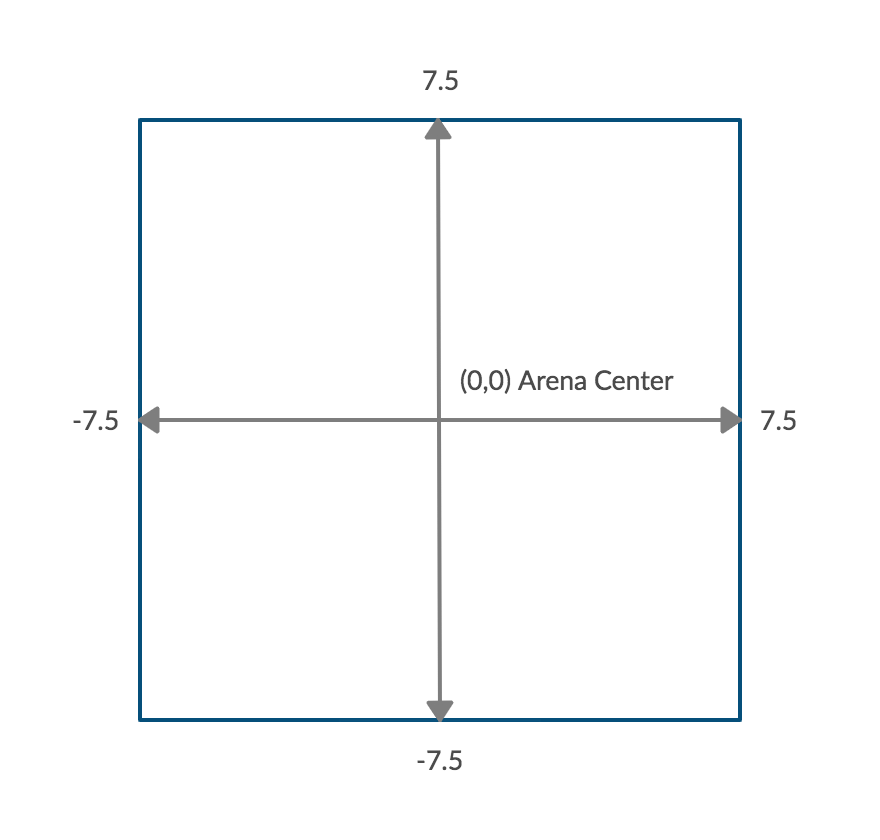
\includegraphics[width=0.45\textwidth]{images/global_ref_frame.png}
  \caption{``Global Odometry'' reference frame maintained by every Swarmie, featuring the arena center, with its collection zone, at the origin. The depiction assumes a $15 \times 15$ meter square arena.}
  \label{fig:global_ref_frame}
\end{figure}

\begin{figure}[ht!]
  \centering
  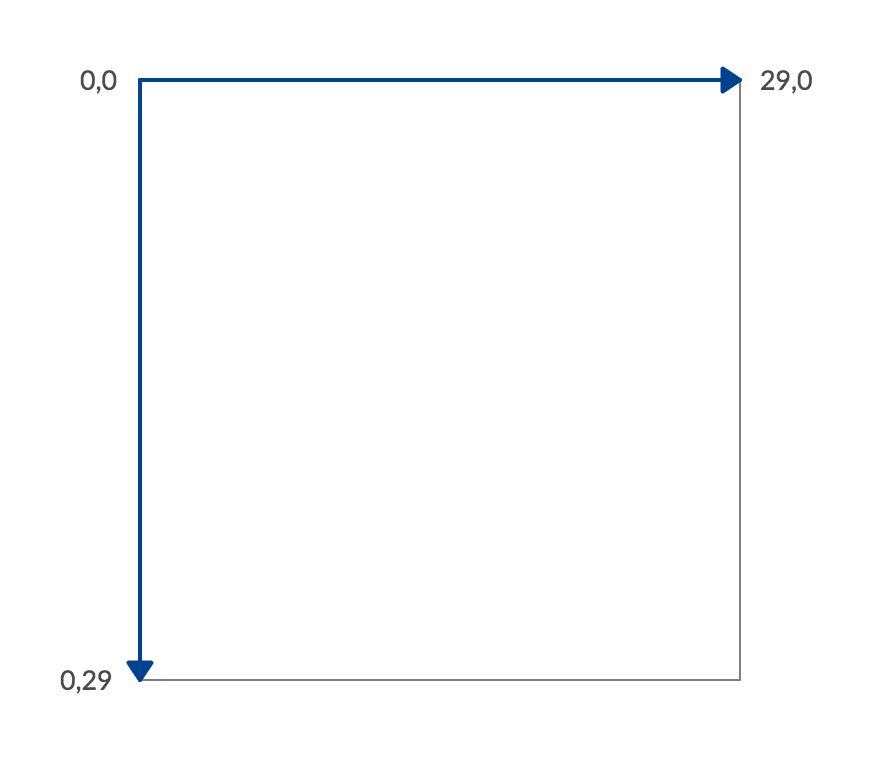
\includegraphics[width=0.45\textwidth]{images/grid_ref_frame.png}
  \caption{``Grid'' reference frame maintained by every Swarmie, featuring the top-left corner of the arena as its origin. The depiction assumes a $30 \times 30$ grid.}
  \label{fig:grid_ref_frame}
\end{figure}

Fused localization readings received by each Swarmie are first converted to the Global Odometry frame by performing a translation from the local odometry frame (which is centered at the Swarmie's starting location). Grid frame transformation is then done by digitizing each Global Odometry axis individually to the range $[0, 29]$ (30 total spaces).

Communication of gross robot position as well as April Cube sightings amongst the swarmies is always done using the Grid reference frame. Furthermore, gross movement around the competition arena done by each Swarmie also uses the Grid reference frame. Only precise robot movement (such as that done to approach a cube or travel to the collection zone) is done using Global Odometry frame coordinates.

\subsection{Action Decomposition}\label{subsec:action_decomp}
Given that both \textbf{Search} and \textbf{Fetch} are very high level actions for a robot to do, even when fully qualified, an action decomposition scheme helps to break down these high level actions into actionable tasks.

At the lowest level of the action decomposition hierarchy are five actions:
\begin{enumerate}
  \item \textbf{Turn} - As the name implies, this action is used to orient the robot so forward motion is toward a specific bearing, measured using Yaw.
  \item \textbf{Drive} - Moves the robot either backwards or forward at a specific speed with no particular location in mind.
  \item \textbf{Approach} - Although this action could be expressed in terms of \textbf{Turn} and \textbf{Drive}, it is done separately in order to gain the most precision while approaching an April Cube.
  \item \textbf{Claw Fingers} - Used to either open or close the Swarmie claws during cube pickup or drop off.
  \item \textbf{Claw Wrist} - Used to either lower or raise the Swarmie claws during cube pickup or drop off.
\end{enumerate}

At a higher level there are five actions that are expressed in terms of the aforementioned lowest-level actions:
\begin{enumerate}
  \item \textbf{Drop Off} - Used to execute an April Cube drop sequence using \textbf{Claw Fingers} and \textbf{Claw Wrist} lower level actions.
  \item \textbf{Move to Cell} - Relocates a Swarmie using Grid reference frame coordinates and $A^*$ path planning using \textbf{Turn} and \textbf{Drive} lower level actions.
  \item \textbf{Move to Global} - Relocates a Swarmie using Global Odometry reference frame coordinates using \textbf{Turn} and \textbf{Drive} actions (with PID loop assisted Yaw maintenance during \textbf{Drive}).
  \item \textbf{Pick Up} - Used to execute an April Cube pickup sequence using \textbf{Claw Fingers} and \textbf{Claw Wrist} lower level actions.
  \item \textbf{Sweep} - Used to sweep the Swarmie's current area for April Cubes using the \textbf{Turn} lower level action.
\end{enumerate}

At the highest level lie the \textbf{Search} and \textbf{Fetch} actions which are expressed exclusively in terms of the aforementioned lower level actions. In order to fully qualify the \textbf{Fetch} action, the location of an April Cube in Grid reference frame coordinates must be specified. In order to fully qualify the \textbf{Search} action, a search quadrant label must be specified. The available search quadrants, along with their respective labels and scanning orientations, is depicted in Figure \ref{fig:search_quads}.

\begin{figure}[ht!]
  \centering
  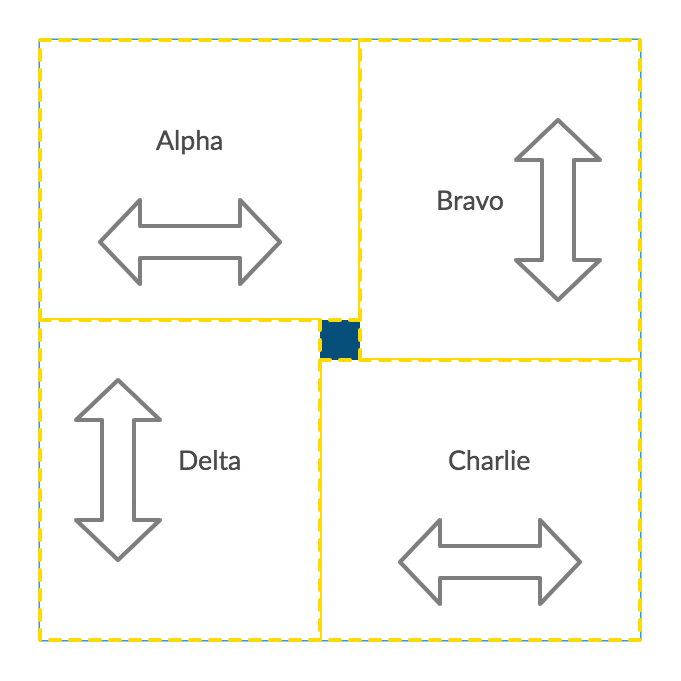
\includegraphics[width=0.45\textwidth]{images/search_quads.png}
  \caption{Depiction of the search quadrants used by the Search action, along with their respective labels and scanning orientations. Those with a left-right orientation scan the area primarily by traveling all the cells in a row before moving on to the next row. Those with an up-down orientation scan the area primarily by traveling all the cells in a column before moving on to the next column. The collection area is shown as the opaque square in the middle.}
  \label{fig:search_quads}
\end{figure}

\subsection{Architecture}\label{subsec:architecture}
As stated in Section \ref{subsec:challenges}, there are several functional components present in the NASA Swarmathon code base that the solution presented in this study will utilize as-is. Thus, the high-level architecture diagram depicted in Figure \ref{fig:architecture} many of the details regarding baseline functionality as well as basic Robot Operating System (ROS) mechanics.

\begin{figure*}[ht!]
  \centering
  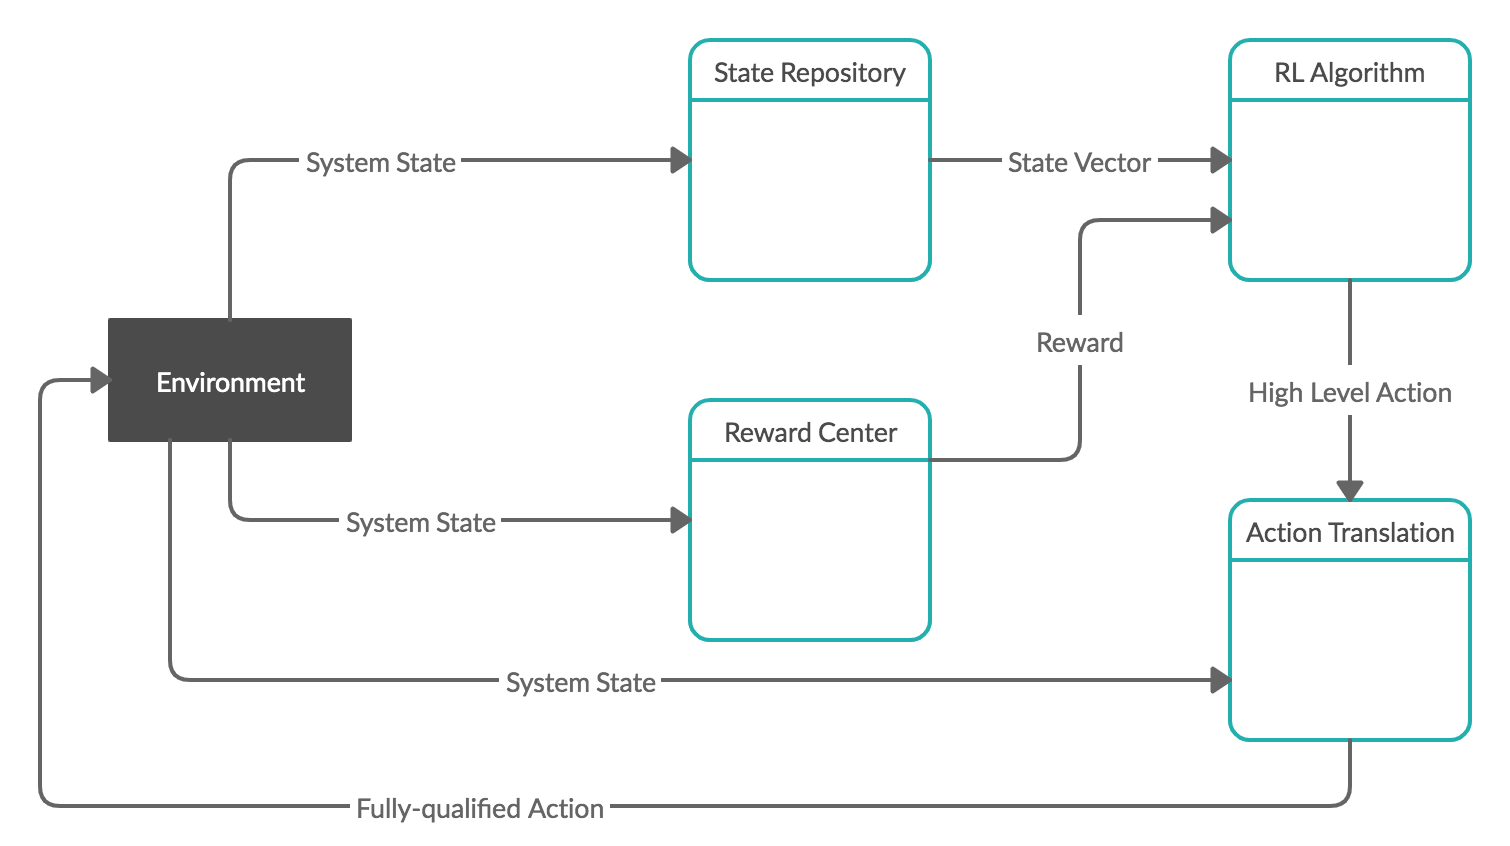
\includegraphics[width=0.9\textwidth]{images/architecture.png}
  \caption{High-level architectural diagram depicting how the RL algorithm and its ancillary components interact with the overall system, primarily via the depiction of data flow between components.}
  \Description{High-level architectural diagram for the Swarmies RL solution.}
  \label{fig:architecture}
\end{figure*}

Among other things, Figure \ref{fig:architecture} makes clear the kind of information that the behavior component requires in order to properly operate. For the sake of simplicity, information flows in the diagram are summarized into top-level categories.

The \textbf{System State} category includes all of the information that the NASA Swarmathon ROS workspace as a whole makes available to each running entity. This information includes elements already available prior to the implementation of the RL logic, as well as information introduced by the RL behavior in order to promote cooperation amongst agents.

Examples of already available information include robot localization messages (such as those resulting from Kalman filter sensor fusion) as well as computer vision (CV) results (such as April Tag sightings).

An example of new information introduced by the RL logic include common reference frame position information derived from local robot localization information. Another example of new information includes April Tag sighting information expressed in a common reference frame. This apparent rebroadcast is necessary because April Tag sightings are in a virtual ``closed circuit'' between the CV logic and the Swarmie that captured the sighting with its own camera.

The \textbf{State Vector} category simply includes the state vector derived from the aforementioned state information. Details of this derivation are available in Section \ref{subsec:state_space}.

The \textbf{Reward} category includes the rewards and penalties as perceived via the available \textbf{System State} information. Further details regarding the reward/penalty information is available in Section \ref{subsec:reward_signal}.

The \textbf{High-Level Action} category represents the ``one-hot'' result as yielded by the RL algorithm (see Section \ref{subsec:action_space}). As is, this result is insufficient to interact with the system, thus there is a need to ``translate'' this high level action into something more useful.

The \textbf{Fully-qualified Action} category represents the transformation of the ``one-hot'' result yielded by RL into something actionable by the environment. The transformation is required since, for example, when the RL algorithm yields a \textbf{Fetch} action, the environment must be told exactly \textit{what} to fetch. In this example, the \textbf{System State} information helps fully-qualify the action by identifying the closest sighted April Cube for collection by the particular Swarmie. Similarly, a \textbf{Search} action submitted to the system must specify exactly \textit{where} to search. The
\textbf{System State} factors here too since it is able to determine which areas are being searched by other agents at any particular time. Selection of a search area takes that information into account in order to promote a broader arena search.

The \textbf{State Repository} is a stateful component that retains information pertaining to last known Swarmie locations, declared actions, and April Cube sightings. The aforementioned subcomponent uses this cached information in order to maintain system state, and provide it to the Swarmie behavior component on demand. Both the RL algorithm and ``Reward Center'' benefit from this service.

\subsection{RL Model}\label{subsec:rl_model}
The Reinforcement Learning (RL) model used in this implementation is at a high level a Double Deep Q-Network (DDQN) that receives the state vector samples as input and outputs the one-hot action vector. The implementation uses a main and ``target'' neural network to assist in training. During training, model goes through the following steps:
\begin{enumerate}
  \item Select and act on an action based on the state of the main neural network.
  \item Save a sample that contains the previous state, action taken, next state, and reward earned in an experience replay buffer.
  \item Once enough of the aforementioned samples are collected, tune the main model by evaluating the actions taken using the ``target'' model.
  \item After a model tuning session, the state of the main network is copied over to the ``target'' network.
\end{enumerate}

Action selection during training is done using an $\epsilon$-Greedy policy where the exploration coefficient $\epsilon$ decays over time in a particular episode. Action selection during non-training runs is done with a basic Greedy policy.

\subsection{Relaxed Environment}\label{subsec:relaxed_env}
Since the focus of this study is the design and evaluation of an RL agent that must choose between \textbf{Search}ing for cubes or \textbf{Fetch}ing them, doing the RL training in an environment with peripheral (albeit important) considerations like kinematics and sensor inaccuracies seemed inappropriate. Thus, a ``Relaxed'' environment was put together in order to facilitate agent design and evaluation.

In this relaxed environment, the following concessions were made to the agent:

\begin{enumerate}
  \item Positioning is always done using the Grid reference frame.
  \item Localization does not degrade over time.
  \item Traversing an occupied grid cell does not disturb any existing April Cubes.
  \item Travel between grid cells is done at a constant speed of 1 cell per time step. Assuming the distance between cells is $0.5$ meters and the time step equivalence of 1 step $\rightarrow$ 2 seconds, this assumes a speed of $0.25 \tfrac{m}{s}$, which is reasonable.
  \item Action hierarchy reduced to five total actions:
  \begin{enumerate}
    \item \textbf{Move} - Move to an adjacent cell in the grid.
    \item \textbf{Pick Up} - Pick up a cube in the current cell.
    \item \textbf{Drop Off} - Drop a cube in the current cell.
    \item \textbf{Search} - Search a quadrant as specified in Figure \ref{fig:search_quads}
    \item \textbf{Fetch} - Fetch a block at a specified cell.
  \end{enumerate}
\end{enumerate}

The relaxed environment is used exclusively for training, whereas the full-blown ROS environment is only used for non-training runs using an already-trained model. Runs done on the relaxed model save the neural network state so it may be restored and used in full-blown ROS runs. Given that the model interface remains constant, with state vectors coming in and action vectors going out, no model adaptation is necessary.

The relaxed environment produces comma-separated value (CSV) data files with a row record for every episode ran. Each record contains the episode number, the number of steps the episode ran for, and the total score achieved during the run (i.e., the number of cubes collected in the ``nest'')

Additionally, in order to properly evaluate the model training performance visually, relaxed model runs generate logs of every move done by the hosted agents. These activity logs are the fed through a visualization tool that presents a pictorial representation of the run. A screenshot produced by the visualization tool is shown in Figure \ref{fig:relaxed_screenshot}. Each cell contains a dark grey number representing the April Cube ``Ground Truth.'' Each swarmie is represented by a colored square over the cells. Cells shaded in pale yellow represent locations where a swarmie has detected the presence of an April Cube. The center is the collection zone with the up to date count of cubes collected. In order to simplify graphical development, the relaxed environment visualization tool was written using the PyGame library.

\begin{figure}[ht!]
  \centering
  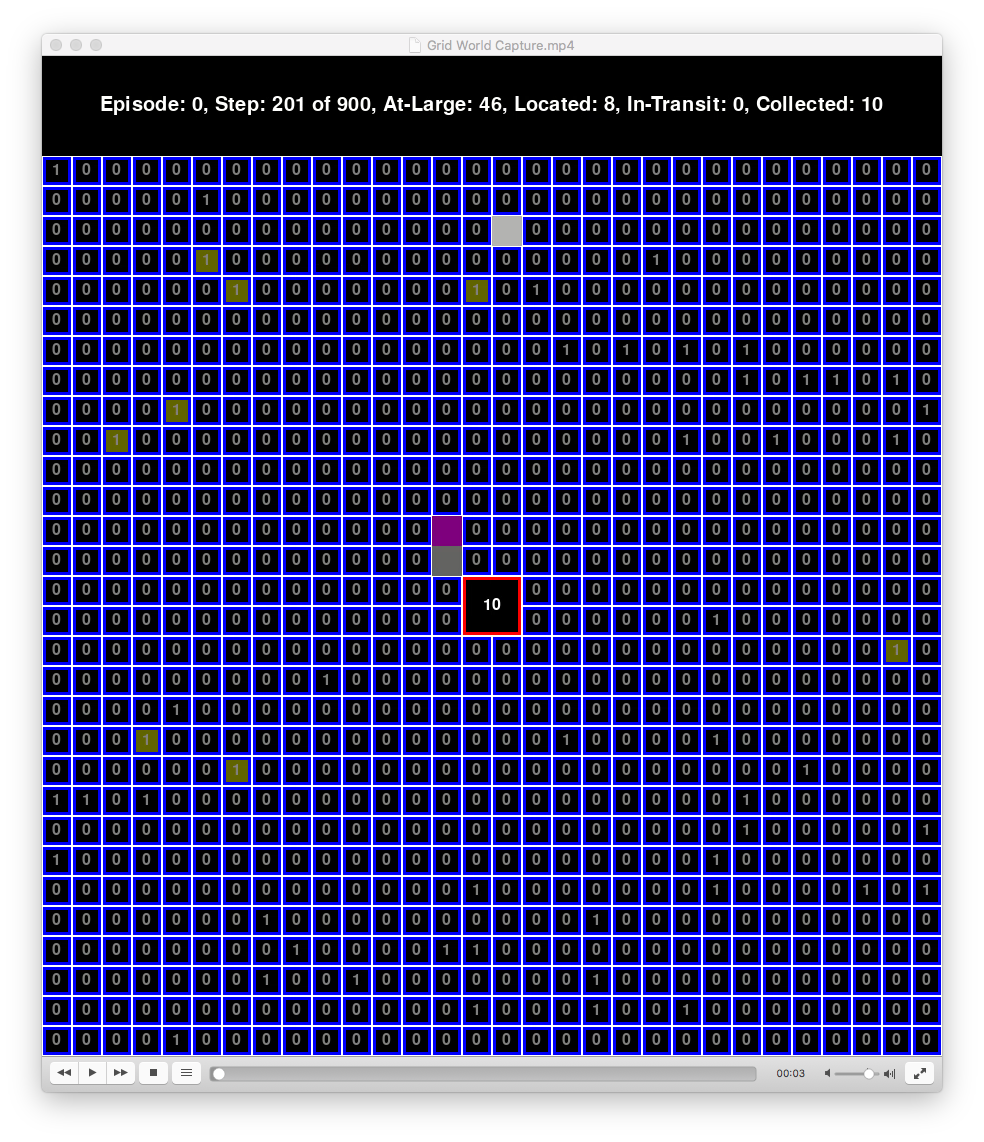
\includegraphics[width=0.45\textwidth]{images/relaxed_screenshot.png}
  \caption{Screenshot of the Relaxed Environment visualization tool used to present the events that transpire during a training session in the relaxed swarmies environment.}
  \label{fig:relaxed_screenshot}
\end{figure}

\section{Experimental Results}\label{sec:results}
The RL training in the Relaxed Environment was done over five (5) sessions, with each session consisting of 100 episode runs. Each episode consisted of a maximum 900 time steps. Once a model was fully trained, its state was ported over to the ROS/Gazebo environment for final evaluation.

Among the five total sessions, there were slight differences that impacted the model's performance in a material manner:
\begin{enumerate}
  \item One run was done without any path deconflicting logic, and with the ``futile fetch'' penalty nullified (labeled ``bravo'').
  \item One run was done with path deconflicting logic, but with the ``futile fetch'' penalty still nullified (labeled ``charlie'').
  \item Three runs were done with both path deconflicting and the ``futile fetch'' penalty enabled (labeled ``delta,'' ``echo,'' and ``foxtrot.'').
\end{enumerate}

The overall score after each episode for each run is depicted in Figure \ref{fig:score_graph}. The first fact that is plainly obvious after inspecting the score graph is that, indeed, the addition of path deconflicting logic (not necessarily related to RL) and the ``futile fetch'' penalty had a material impact on the model's performance. Runs \textit{Delta}, \textit{Echo}, and \textit{Foxtrot} appear nearly identical in scoring performance, which is to be expected given their identical starting configurations.

\begin{figure}[ht!]
  \centering
  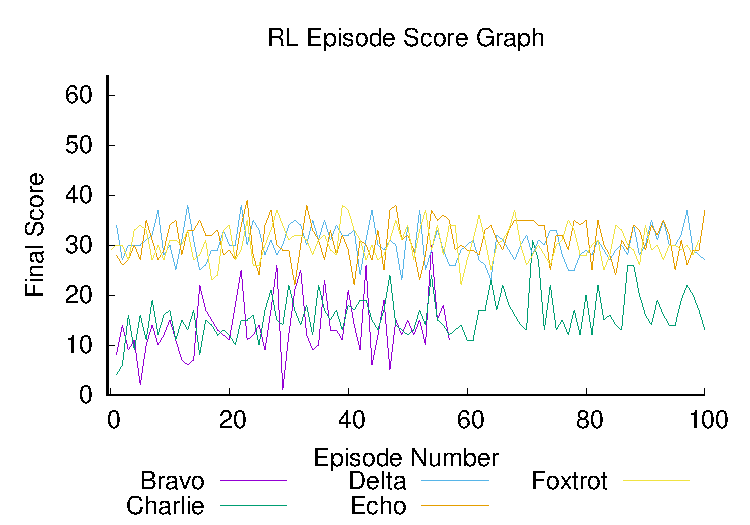
\includegraphics[width=0.45\textwidth]{images/score_graph.pdf}
  \caption{Overall score graph for all five training runs of the Swarmie RL model.}
  \label{fig:score_graph}
\end{figure}

Another surprising fact evident when examining Figure \ref{fig:score_graph} is the lack of a ``training slope'' in runs \textit{Delta}, \textit{Echo}, and \textit{Foxtrot}. It appears that, after the very first episode, the model achieved peak performance. Such behavior was later confirmed when observing the training run replays in the activity log visualization tool (Figure \ref{fig:relaxed_screenshot}). Runs \textit{Bravo} and \textit{Charlie} do exhibit a bit of a training slope that seems to settle after episode 40 or so.

Given the similar performance between \textit{Bravo} and \textit{Charlie}, and the fact that the only difference between them was the addition of path deconflicting logic in the \textit{Charlie} run, it would seem that the ``futile fetch'' penalty had a much more appreciable effect on the model performance. Another impact of the ``futile fetch'' penalty is the apparent lower variance of the score graphs for runs that employ it, compared to those that do not.

Although an average performance for the model that hovers in the low-mid 30's seems somewhat lackluster, it should be noted that two factors made achieving a perfect score in an episode next to impossible: the episode length and the arena size.

The episode length was established as 900 steps given that every time step is equivalent to two seconds, and a typical Swarmathon match lasts only 30 minutes ($1,800$ seconds). Considering that a $30 \times 30$ grid possesses 900 distinct cells (save for the four occupied by the collection zone), it would require just about an entire episode's number of steps to visit every cell at least once. That said, the exploration patterns written in the Swarmie logic are not perhaps the most efficient, thus leaving the possibility for improvement by future work.

Unfortunately, the relative success observed in the relaxed environment did not translate well into the ROS/Gazebo environment. Although the translation of state information into state vectors, as well as the translation from action vectors into actionable tasks, was quite successful, there were a lot of other concerns not related to RL that impeded the progress of the model's actions.

First and foremost was the problem related to path deconflicting. Although the ultrasonic sensors built into the Swarmie robots were useful in avoiding collisions, actually completing the deconflicting requires the re-planning of a swarmie's path. Swarmies traveling perpendicular to each other were not much trouble in this regard, but there were plenty of instances where Swarmies stood ``head to head.'' In such a situation, deconflicting is more difficult. Path replanning using the opposite Swarmie as a temporary obstacle was implemented in the \textbf{Move to Cell} action, but that is the only action that actually employs a path plan. The others were forced to simply stop when the ultrasonic sensors registered an obstacle nearby. Path deconflicting in the relaxed environment was implemented by having both swarmies that were facing ``head-to-head'' to turn right. Doing so automatically put them in a different path right away, and they were able to resume their chosen action.

Another emergent behavior that posed a problem in the ROS/Gazebo environment was the introduction of sensor drift. Since the GPS sensor is realistically emulated to exhibit discontinuous, rather severe jumps (some measuring almost 2 meters), the only measurement that seemed appropriate to use for positioning was the fused Odometer/IMU reading. In the beginning of the runs, the position information yielded by this sensor combination was quite adequate. However, as time advanced, and especially after the robots collided while attempting conflicting actions, the sensors drifted to the point of being nearly useless. As far as the robot behavior logic was concerned, the mobility commands were being carried out appropriately. However, as it is evident in the video that accompanies this report, the true performance was completely different.

Finally, one aspect of the relaxed environment that did not translate well to the ROS/Gazebo environment concerned the actual collection of the April Cubes. In the relaxed environment, once a Swarmie made the decision to pick up a cube, it succeeded without question. In the ROS/Gazebo environment, entire approach sequences had to be engineered outside the realm of RL in order to properly collect a cube. In addition, once a cube was collected, the Swarmie sensor package did not reliably provide positive indication that the collection had been a success. The only positive indication available was the recognition of the cube's April Tag at a very close proximity from the camera. There were a lot of times when, although the Swarmie did succeed in picking up a cube, the lack of this positive verification led it to believe the pickup had failed.

Although a proper relaxed environment run was able to achieve collection scores in the 30's, the ROS/Gazebo environment was only able to properly collect one cube. It should be noted, however, that due to performance considerations, the ROS runs were done with only 16 April Cubes in the field, whereas the relaxed environment runs were done with 64 cubes.

The video presentation that accompanies this report contains captures of both the relaxed environment runs and a ROS/Gazebo run. It is available at the link that follows:

\begin{verbatim}
  https://youtu.be/TmWFqBy5SK0
\end{verbatim}

The source code for the ROS/Gazebo implementation of the RL agent behavior is at the following link:

\begin{verbatim}
  https://github.com/rjnieves/SwarmiesRL
\end{verbatim}

The source code for the Relaxed Environment training application is at the following link:

\begin{verbatim}
  https://github.com/rjnieves/RelaxedSwarmiesRL
\end{verbatim}

And finally, the source code for the Relaxed Environment activity log visualization tool is at the following link:

\begin{verbatim}
  https://github.com/rjnieves/VizSwarmies
\end{verbatim}

All of the runs done to support this study were done on a workstation with the specifications shown in Table \ref{tab:workstation_specs}.

\begin{table}
  \centering
  \caption{Pertinent specifications for the workstation used to run the experiments documented in this study.}
  \label{tab:workstation_specs}
  \begin{tabular}{|l|l|}
    \hline\hline
    \textbf{CPU} & Intel Core i7-7700 \\
    \hline
    \textbf{GPU} & NVIDIA GeForce GTX-970 \\
    \hline
    \textbf{OS} & Ubuntu 16.04 \\
    \hline
    \textbf{ROS} & Kinetic \\
    \hline
    \textbf{Python} & 2.7.16 \\
    \hline
    \textbf{TensorFlow} & 1.14 \\
    \hline
    \textbf{Keras} & 2.2.4 \\
    \hline
    \textbf{PyGame} & 1.9.6 \\
    \hline\hline
  \end{tabular}
\end{table}

\section{Conclusion}\label{sec:conclusion}
Although the performance of the Multi-Agent Reinforcement Learning (RL) implementation in a realistic simulation environment was not as originally expected, the test results of the same model under a relaxed environment provide evidence that performance can definitely be improved and that the use of RL can be a valuable boon for this kind of problem. Focusing exclusively on the algorithm in the relaxed environment showed that an RL agent can quickly come up to speed on such a foraging task, and perform reasonably well. Given the complexity of the problem, the relatively low dimensionality of the algorithm's state representation demonstrate that there is plenty of room to grow for future endeavors.

There were several aspects of the overall foraging problem that were not properly addressed in this study given its primary focus, but it stands to reason that dedicating efforts to shoring up these deficiencies could yield even better results than those presented in this study.

Focused exclusively on the RL algorithm, the state vector did not contain any information regarding where or how much of the competition arena had been already searched. Engineering a way to include such information into the state vector, with the corresponding rewards and penalties, should yield a much more efficient use of the time alloted to the Swarmies in their hunt for April Cubes. In the implementation done for this study, selection of a search quadrant was done by pure random selection, with some help that avoided conflicts among the Swarmies that chose to go searching.

Focusing on the peripheral yet important issues of robot mobility and localization, there is plenty of room for improvement for future researchers. From engineering a more clever localization scheme (compared to the grid discretization done in this study), to implementing better compensation for sensor drift, there were a lot of areas that performed poorly and, thus, impacted the performance of the RL implementation. It is not unreasonable to think that an entire study could be done in these subjects alone.

The Swarmie robots, as currently built, could use some enhancements in their sensor package too. Perhaps it was economics that limited their sensor suite to
\begin{enumerate*}[(1)]
  \item an odometer,
  \item an IMU,
  \item an inexpensive USB camera with limited visual range, and
  \item ultrasonic sensors only focused in the forward direction.
\end{enumerate*}
Given more sensors to lean on would have possibly aided in establishing a better situation awareness, and quite possibly have eliminated the need to engineer the state space vector using domain information in favor of a more generic model such as those employed to learn Atari games via multi-layer networks.

Other opportunities where RL could prove useful to this domain is the application of individual RL to some of the more demanding tasks levied on the Swarmies. Perhaps the layering of individual RL models that control April Cube individual behaviors such as approach and pickup, combined with the higher level RL model that calls out the \textbf{Search} and \textbf{Fetch} actions could yield a better performing system. Several of the actions listed in Section \ref{subsec:action_decomp} are prime candidates for implementation using RL, even if it veers from the multi-agent variety attempted in this study.

In the end, however, this study has been an enormous learning opportunity for the author. An experience that has generated an elevated level of respect for those that work in robotics on a daily basis.

\bibliographystyle{ACM-Reference-Format}
\bibliography{swarmies_rl}

\end{document}
